\quad\quad\quad\quad{\it by K. Becker, C. Bertella, M. Bonvini, A. Calderon Tazon, J. Campbell, F. Caola, X. Chen,
P. Francavilla, S. Frixione, R. Frederix, T. Gehrmann, N. Glover, Y. Haddad, V. Hirschi, A. Huss, S. Jones, 
A. Karlberg, M. Kerner, J. Lindert, G. Luisoni, G. Marchiori, S. Marzani, A. Massironi, B. Mistlberger,
P. Monni, M. Moreno Llacer, A. M\"uck, C. Palmer, C. Pandini, L. Perrozzi, S. Pozzorini, E. Re, L. Reina,
H.S. Shao, L. Simon, B. Stieger, V. Theeuwes, F. Tramontano and M. Zaro}

 
\subsubsection{Introduction}

Cross-section predictions for the high-energy (HE) LHC, and their associated theoretical uncertainties, are discussed and shown in
Section~\ref{sec:he-lhc}. Predictions are computed for a proton-proton collider with a $pp$ centre-of-mass
energy $\sqrt{s}=27$~TeV and use a Higgs
boson mass of $m_H=125.09 \pm 0.5$~GeV.   All other parameters are taken from YR4~\cite{deFlorian:2016spz},
with exceptions noted where they are important.  
Projections of progress towards a reduction in theoretical uncertainties, on the timescale
of the high-luminosity (HL) LHC (3~ab$^{-1}$ of $pp$ collisions at $\sqrt{s}=14$~TeV), are discussed in Section~\ref{sec:hl-lhc}. 
Tables summarizing a detailed study of the dependence of the gluon-fusion cross section on the mass of the Higgs boson
are presented in Section~\ref{sec:ggFmhdep}.

\subsubsection{Cross sections for 13, 14 and 27 TeV HE-LHC}
\label{sec:he-lhc}

This section provides updated cross-sections for the LHC operating at
energies of $13$, $14$ and $27$~TeV. All predictions~\cite{HXSWGwiki} include the latest 
theoretical input and supersede the older results in YR4~\cite{deFlorian:2016spz}.

\subsubsubsection{Gluon fusion}
\label{sec:he-lhc-ggF}
In this section we document cross section predictions for a standard
model Higgs boson produced through gluon fusion in 27~TeV $pp$ collisions.  To
derive predictions we include contributions based on perturbative
computations of scattering cross sections as studied in
Ref.~\cite{Anastasiou:2016cez}.  We include perturbative QCD
corrections through next-to-next-to-next-to-leading order (N$^3$LO), electro-weak (EW) and approximated mixed
QCD-electro-weak corrections as well as effects of finite quark
masses. The only modification with respect to YR4~\cite{deFlorian:2016spz} is that we
now include the exact N$^3$LO heavy top effective theory cross section of
Ref.~\cite{Mistlberger:2018etf} instead of its previous approximation. The
result of this modification is only a small change in the central values and
uncertainties. To derive theoretical uncertainties we follow the
prescriptions outlined in Ref.~\cite{Anastasiou:2016cez}.
We use the following inputs:
\begin{equation}
\begin{array}{c  c}
\hline
\text{E}_\text{CM} & 27~\text{TeV} \\
\text{m}_\text{t}(\text{m}_\text{t}) & 162.7~\text{GeV} \\
\text{m}_\text{b}(\text{m}_\text{b}) & 4.18~\text{GeV} \\
\text{m}_\text{c}(3 \text{ GeV}) & 0.986~\text{GeV} \\
\alpha_\text{S} (m_Z) & 0.118  \\
\text{PDF} & \text{PDF4LHC15\_nnlo\_100}\text{~\cite{Botje:2011sn}}\\
\hline
\end{array}
\end{equation}
All quark masses are treated in the $\overline{\text{MS}}$ scheme. To derive numerical predictions we use the program \texttt{iHixs}~\cite{Dulat:2018rbf}.

Sources of uncertainty for the inclusive Higgs boson production cross section have been assessed recently in refs.~\cite{Anastasiou:2016cez,Harlander:2016hcx,Bonvini:2016frm,deFlorian:2016spz}. 
Several sources of theoretical uncertainties were identified.
\begin{figure}[h]
\begin{center}
    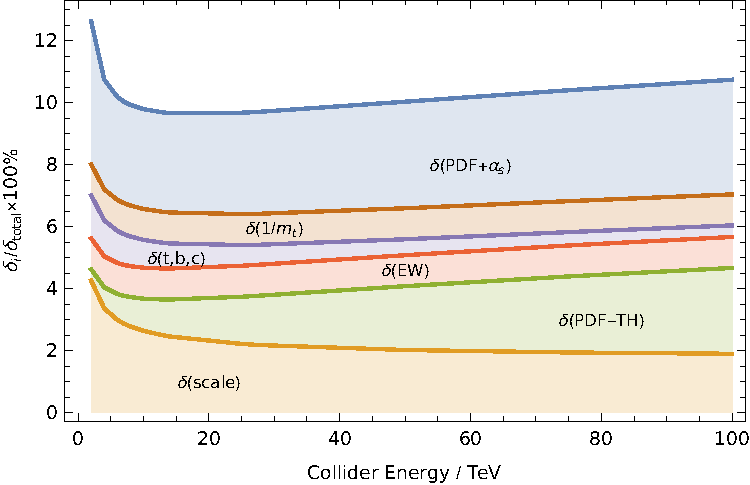
\includegraphics[width=0.7\textwidth]{\main/section2/plots/error_plot.pdf}
    \caption{
    The figure shows the linear sum of the different sources of relative uncertainties as a function of the collider energy. 
    Each coloured band represents the size of one particular source of uncertainty as described in the text.
    The component $\delta(\text{PDF}+\alpha_S)$ corresponds to the uncertainties due to our imprecise knowledge of the strong coupling constant and of parton distribution functions combined in quadrature.
        \label{fig:errorplot}}
        \end{center}
\end{figure}
\begin{itemize}
\item Missing higher-order effects of QCD corrections beyond N$^3$LO ($\delta(\text{scale})$).
\item Missing higher-order effects of electro-weak and mixed QCD-electro-weak corrections at and beyond $\mathcal{O}(\alpha_S \alpha)$ ($\delta(\text{EW})$).
\item Effects due to finite quark masses neglected in QCD corrections beyond NLO  ($\delta(\text{t,b,c})$ and $\delta(1/m_t)$).
\item Mismatch in the perturbative order of the parton distribution functions (PDF) evaluated at NNLO and the perturbative QCD cross sections evaulated at N$^3$LO ($\delta(\text{PDF-TH})$).
\end{itemize}
In the tables the linear sum of the effect of those uncertainties
is referred to as $\delta(\text{theory})$.  In addition, the imprecise
knowledge of the parton distribution functions and of the strong coupling
constant play a dominant role.  The individual size of these
contributions can be seen in fig.~\ref{fig:errorplot} as a function of
the collider energy~\cite{Dulat:2018rbf}.  As can be easily inferred
the relative importance of the different sources of uncertainty is
impacted only mildly by changing the centre of mass energy from $13$
TeV to $27$ TeV.  Inclusive cross sections for
$m_H=125.09$ GeV are given in Table~\ref{tab:results}. As noted above, the
exact treatment of N$^3$LO QCD corrections results in a
small shift in the cross-section at 13~TeV, relative to the YR4 resut, and
a slight reduction in the overall theoretical uncertainty.
\begin{table}[!h]
\normalsize\setlength{\tabcolsep}{2pt}
\begin{center}
    \begin{tabular}{rrrrr}
        \toprule
        \multicolumn{1}{c}{$\sqrt{s}$}&
        \multicolumn{1}{c}{$\sigma$}&
        \multicolumn{1}{c}{$\delta(\textrm{theory})$}&
        \multicolumn{1}{c}{$\delta(\textrm{PDF})$}&
        \multicolumn{1}{c}{$\delta(\alpha_s)$}\\
        \midrule
13 TeV & 48.61 pb & ${}^{+2.08\textrm{pb}}_{-3.15\textrm{pb}}\,\left({}^{+4.27\%}_{-6.49\%}\right) $ & $\pm\,0.89\,\textrm{pb}\,(\pm\,1.85\%)$ & ${}^{+1.24\textrm{pb}}_{-1.26\textrm{pb}}\,\left({}^{+2.59\%}_{-2.62\%}\right) $ \\%\midrule
14 TeV & 54.72 pb & ${}^{+2.35\textrm{pb}}_{-3.54\textrm{pb}}\,\left({}^{+4.28\%}_{-6.46\%}\right) $ & $\pm\,1.00\,\textrm{pb}\,(\pm\,1.85\%)$ & ${}^{+1.40\textrm{pb}}_{-1.41\textrm{pb}}\,\left({}^{+2.60\%}_{-2.62\%}\right) $ \\%\midrule
27 TeV & 146.65 pb & ${}^{+6.65\textrm{pb}}_{-9.44\textrm{pb}}\,\left({}^{+4.53\%}_{-6.43\%}\right) $ & $\pm\,2.81\,\textrm{pb}\,(\pm\,1.95\%)$ & ${}^{+3.88\textrm{pb}}_{-3.82\textrm{pb}}\,\left({}^{+2.69\%}_{-2.64\%}\right) $ \\
   \bottomrule
    \end{tabular}
    \caption{Gluon fusion Higgs boson production cross sections and uncertainties as a function of the $pp$ collider energy.\label{tab:results}}
\end{center}
\end{table}

Improving substantially on any of the current
sources of uncertainty represents a major theoretical challenge that
should be met in accordance with our ability to utilise said precision
and with experimental capabilities. 
The computation of subleading mass and EW corrections is
currently being addressed by several groups, and therefore it is
likely to be achieved in the next decade. Although such computations
will allow for a better control over some sources of uncertainty,
their final impact on the full theoretical error is likely to be
moderate as current estimates indicate.
Another source of error that might improve in the forthcoming years is
that related to the parton densities. In particular, the extraction of
N$^3$LO PDFs would lead to the disappearance of the PDF-TH
uncertainty. Similar considerations apply to the error on the strong
coupling constant, that will be reduced due to more accurate
extractions. Overall, the above progress would ultimately lead to a
notable reduction of the uncertainties of Figure~\ref{fig:errorplot}.

It is obvious that the future precision of experimental measurement of Higgs boson properties will challenge the theoretical community.
Achieving a significant improvement of our current theoretical understanding of the Higgs boson and its interactions will inspire us to push the boundaries of our capabilities to predict and extract information.
New ways of utilising quantum field theory in our endeavours have to be explored and our perturbative and non-perturbative understanding of hadron scattering processes has to evolve substantially. 
It is clear that this exciting task can only be mastered by a strong and active collider phenomenology community.
 
The dependence of the inclusive gluon-fusion cross-section on the Higgs boson mass at $\sqrt{s}=14$ and 27~TeV
is detailed at the end of this note in Section~\ref{sec:ggFmhdep}.


\subsubsubsection*{Impact of future precision of parton distribution function}
It is a tantalising question to ask by how much one of the largest sources of uncertainty - the imprecise knowledge of PDFs - would be reduced if already all future LHC data were available.
To this end a study was performed in ref.~\cite{Khalek:2018mdn} that uses simulated future data with accordingly shrunken statistical uncertainties to constrain parton distribution functions.
The authors used pseudo data corresponding to measurements of ATLAS, CMS and LHCb for key precision processes after $3 ab^{-1}$ of integrated luminosity were collected at the High-Luminosity LHC at 14 TeV.
They then performed a new fit according to the PDF4LHC15 framework~\cite{Botje:2011sn} and studied the implications of their analysis.
The resulting PDFs are readily available and can be used in order to estimate the impact of this future data on specific observables. 
Three scenarios were considered in this study that assume that experimental systematic uncertainties will shrink at different levels relative to the 8 TeV run of the LHC.
Scenario 1, scenario 2 and scenario 3 assume that the future systematic uncertainty will be equal, shrunk by a factor $0.7$ or a factor of $0.4$ w.r.t to the 8 TeV run respectively.

Evaluating the inclusive Higgs boson production cross section with this simulated PDFs results in the PDF uncertainties summarised in Tab.~\ref{tab:PDFuncert}.
Note, that the central values stay unchanged and all other uncertainties are not afflicted by the change of PDFs.
\begin{table}[!h]
\normalsize\setlength{\tabcolsep}{2pt}
\begin{center}
    \begin{tabular}{rrrrr}
        \toprule
        \multicolumn{1}{c}{$\textrm{E}_{\textrm{CM}}$}&
        \multicolumn{1}{c}{Current  }&
        \multicolumn{1}{c}{Scenario 1 }&
        \multicolumn{1}{c}{Scenario 2}&
        \multicolumn{1}{c}{Scenario 3} \\
        \midrule
13 TeV & $ \pm 1.85 \% $ & $\pm 0.78 \%$ & $\pm 0.69\%$ & $\pm 0.59\%$ \\\midrule
14 TeV & $ \pm 1.85 \% $ & $\pm 0.78\%$ & $\pm 0.68\%$ & $\pm 0.58\%$ \\\midrule
27 TeV & $ \pm 1.95 \%$  & $\pm 0.81\%$ & $\pm 0.72\%$ & $\pm 0.61\%$ \\\midrule
    \end{tabular}
    \caption{Uncertainty due to imprecise knowledge of PDFs estimated with current and simulated future PDFs for different scenarios and at different collider energies.\label{tab:PDFuncert}}
\end{center}
\end{table}
Even the most pessimistic scenario leads to a reduction of the PDF uncertainty by factor of two. 
However, this projections should be viewed only as a first estimate for the determination of PDFs from future measurements.
Predicting the future development and correlation of systematic experimental uncertainties is non trivial and may differ strongly from observable to observable. 
PDF uncertainties may in the future also be adversely impacted by a more accurate treatment of theoretical uncertainties in the predictions of cross sections that serve as input for PDF extraction.
Data incompatibilities may occur for various reasons.
It is clear that an understanding of the structure of the proton at percent level accuracy is clearly a formidable task and rightly deserves significant research in the future.




\subsubsubsection*{Impact of threshold and high-energy
  corrections}
Recently, Ref.~\cite{Bonvini:2018ixe} has performed a study of the
effects of simultaneous threshold and high-energy (small Bjorken $x$)
resummations on the inclusive Higgs boson production cross section. In this brief
section we summarise the main conclusions, while the numerical results
will be discussed in the following section. For more details we refer
the reader to Ref.~\cite{Bonvini:2018ixe}:
\begin{enumerate}
\item At different collider energies, it was found that the impact of
  threshold resummation amounts to about $+1\%$ on top of the N$^3$LO
  cross section~\cite{Bonvini:2016frm}. The size of this effect is
  compatible with other estimates of the size of missing higher-order
  corrections.
\item Conversely, the inclusion of small-$x$ resummation was found to
  increase the cross section by about one percent at $13$~TeV, and by
  about $3\%-4\%$ at $27$~TeV, with respect to the N$^3$LO
  prediction. The correction grows even larger at higher 
  energies, reaching about $+10\%$ for a $100$~TeV $pp$ collider. The
  inclusion of high-energy resummation affects differently the
  perturbative coefficient functions and the parton densities.
\begin{itemize}
\item The effect on the coefficient functions is very moderate, and
  remains below the $1\%$ level for different collider energies. This
  indicates that the production of a Higgs boson at present and future
  colliders does not probe very small values of the momentum fraction
  at which the coefficient functions are evaluated.
  In turn, this implies that currently and at future colliders PDFs are probed at intermediate values of x.

\item The parton densities receive a large correction from small-$x$
  resummation. Its effect is twofold: on one hand, the {\it evolution}
  of the gluonic density is modified by the inclusion of small-$x$
  effects, and at average values of $x$ probed in Higgs production
  this leads to a moderate effect on the parton densities at $m_H$
  (cf. Fig. 2.2 of Ref.~\cite{Ball:2017otu}). On the other hand, the
  PDFs used in the double-resummed prediction of
  Ref.~\cite{Bonvini:2018ixe} (\verb+NNPDF31sx_nnlonllx_as_0118+
  \cite{Ball:2017otu}) include small-$x$ data from HERA, which
  Ref.~\cite{Ball:2017otu} observes to require high-energy resummation
  for the fit to be robust. The fixed-order prediction of
  Ref.~\cite{Bonvini:2018ixe} instead uses a PDF set which fits the
  small-$x$ HERA data without including high-energy resummation
  (\verb+NNPDF31sx_nnlo_as_0118+ \cite{Ball:2017otu}).  This results
  in sizeable differences in the parton distribution functions and
  drives the large correction to the N$^3$LO total cross section
  observed in Ref.~\cite{Bonvini:2018ixe}.
\end{itemize}
\end{enumerate}
Summarising, the sizeable corrections to the N$^3$LO prediction due to
high-energy resummation observed in Ref.~\cite{Bonvini:2018ixe} are,
to a large extent, due to the need for high-energy resummation in the
PDF fit which are necessary to get a reliable description of small-$x$
HERA data.  Performing a fit without high energy resummation results
in considerable tension with respect to low $Q^2$ HERA data.  In order
to corroborate these findings, and assess precisely the effect of
high-energy resummation on parton distribution fits, it is important
to make progresses in the theoretical knowledge of small-$x$
dynamics. Furthermore, it would be desirable to include additional
small-$x$ collider data in the fits of parton distributions.  We would
like to encourage the PDF and theory community to further investigate
these effects in view of future high energy colliders.



\subsubsubsection*{Predictions for double-resummed cross
  section}

The setup is the same of the YR4 ($m_H=125$~GeV, $m_t=172.5$~GeV,
$m_b=4.92$~GeV, $m_c=1.51$~GeV, $\as(m_Z^2)=0.118$,
$\muf=\mur=m_H/2$), with the only difference being that we do not use
PDF4LHC but the 
\verb+NNPDF31sx_nnlonllx_as_0118+ set of
Ref.~\cite{Ball:2017otu}.  Since these resummed PDFs are available for
a single value of $\as$, we could not compute the $\as$ uncertainty in
our result. The results are collected in Tab.~\ref{tab:xsec1}.

For each value of the collider energy, we give the full
N$^3$LO+N$^3$LL+LL$x$ cross section which includes top, bottom and
charm contributions (as discussed in Ref.~\cite{Bonvini:2018iwt}) and
EW corrections included in the complete factorization approach, i.e.\
as a $+5\%$ contribution.  The breakdown of the individual terms
contributing to the cross section (the main contribution assuming only
top runs in the loop, the bottom+charm correction, and the EW
correction) is presented in the third column.  In the next columns, we
present various sources of uncertainties,
following Ref.~\cite{Bonvini:2018ixe}:
\begin{itemize}
\item Missing higher-order uncertainty (scale uncertainty)
  $\delta_{\rm scale}^{\rm 42var}$. It is the envelope of standard
  7-point scale variations for each of the subleading variations of
  threshold resummed contributions, resulting in a total of 42
  variation.

\item PDF uncertainty $\delta_{\rm PDFs}$. This is the standard NNPDF
  Monte Carlo replica uncertainty, but it does not contain the $\as$
  uncertainty, as previously discussed.

\item Subleading small-$x$ logarithms uncertainty
  $\delta_{\rm subl.logs}$. This uncertainty is computed as described
  in Refs.~\cite{Bonvini:2018ixe,Bonvini:2018iwt}, and it likely
  overestimates the effect of subleading contributions in the
  coefficient functions. However, as argued in
  Refs.~\cite{Bonvini:2018ixe,Bonvini:2018iwt}, this uncertainty can
  be considered as an estimate of the uncertainty from subleading
  contributions in the PDFs. In this respect, this provides an
  alternative to the uncertainty from missing higher-order PDFs
  adopted in YR4, which should thus not be included.
\end{itemize}
Additional uncertainties from missing $1/m_t^2$ effects, missing
bottom+charm effects and subleading EW effects should be included
according to the YR4 prescription.  Since the N$^3$LO heavy-top result
is matched to the exact small-$x$ according to the construction of
Ref.~\cite{Bonvini:2018iwt}, the ``truncation of the soft expansion''
uncertainty discussed in YR4 should not be considered.

Finally, in the last column of the table we present the ratio of our
resummed result with a purely fixed-order N$^3$LO cross section
obtained with the same settings but using the NNLO parton distribution
functions 
\verb+NNPDF31sx_nnlo_as_0118+ of Ref.~\cite{Ball:2017otu}.  This is
useful to understand how large the effect of resummation(s) in our
prediction is.  We see in particular that the effect (of small-$x$
resummation) grows with the collider energy, reaching $4.6\%$ at
the HE-LHC.  For any of the scales, approximately $+1\%$ of the effect of
resummations is due to threshold resummation (in the coefficient
functions), while the rest of the effect is due to small-$x$
resummation, which mostly comes from the PDFs (see
Ref.~\cite{Bonvini:2018ixe}) as discussed in the previous subsection.
\begin{table*}[t!]
 \centering
 \begin{tabular}{r cc ccc c}
 \toprule
   \multicolumn{1}{c}{$\sqrt{s}$}
   & $\sigma_\text{N$^3$LO+N$^3$LL+LL$x$}$ & $=\sigma_t+\Delta\sigma_{bc}+\Delta\sigma_{\rm EW}$
   & $\delta_{\rm scale}^{\rm 42var}$ & $\delta_{\rm PDFs}$ & $\delta_{\rm subl.logs}$
   & $\frac{\sigma_\text{N$^3$LO+N$^3$LL+LL$x$}}{\sigma_\text{N$^3$LO}}$ \\
\midrule
  13~TeV & $ 48.93$~pb & $( 49.26 -2.66+  2.33)$~pb & ${}_{ -3.8}^{+ 4.0}\%$ & $\pm 1.2\%$ & $\pm 1.8\%$ & $ 1.020$ \\[1ex]
  14~TeV & $ 55.22$~pb & $( 55.56 -2.96+  2.63)$~pb & ${}_{ -3.8}^{+ 4.0}\%$ & $\pm 1.1\%$ & $\pm 1.9\%$ & $ 1.023$ \\[1ex]
  27~TeV & $ 151.6$~pb & $( 151.6  -7.2+   7.2)$~pb & ${}_{ -4.0}^{+ 4.0}\%$ & $\pm 1.0\%$ & $\pm 2.3\%$ & $ 1.046$ \\
  \bottomrule
 \end{tabular}
 \caption{Values of the N$^3$LO+N$^3$LL+LL$x$ gluon-fusion cross section
   for selected values of the $pp$ collision energy and for a Higgs boson mass $m_H=125$~GeV.
   We use the NNPDF31sx PDFs with $\as(m_Z^2)=0.118$, $\mt=173$~GeV, $\mbottom=4.92$~GeV and $\mcharm=1.51$~GeV.}
 \label{tab:xsec1}
\end{table*}



 

\subsubsubsection{Vector boson fusion}
\label{sec:he-lhc-VBF}
The vector-boson fusion (VBF) cross sections are computed with the
same settings as in YR4 and reported in Tab.~\ref{tab:vbf_xsec}. The
description of the setup can be found in the YR4 itself. The EW and photon cross sections have
been computed using the
\texttt{LUXqed\_plus\_PDF4LHC\_nnlo\_100}~\cite{Manohar:2016nzj,Manohar:2017eqh}
PDF set and hence the 13 and 14 TeV cross sections differ slightly
from those reported in the YR4, where
\texttt{NNPDF23\_nlo\_as\_0118\_qed}~\cite{Ball:2013hta} was used
instead. The QCD cross section was computed at NNLO with
proVBFH~\cite{Cacciari:2015jma,Dreyer:2016oyx}, while the EW and
photon contributions have been computed at NLO with
HAWK~\cite{Ciccolini:2007jr,Ciccolini:2007ec,Denner:2014cla}.

\begin{table}
\centering
\begin{tabular}{ccccccc|c}
\toprule
$\sqrt{s}$~[TeV] & $\sigma^{\rm VBF}$~[fb] & $\Delta_{\mathrm{scale}}$~[\%] &
$\Delta_{\mathrm{PDF\oplus\alpha_s}}$~[\%] &
$\sigma_{\rm NNLO}^{\rm DIS}$~[fb] & $\delta_{\rm ELWK}$~[\%] & $\sigma_{\gamma}$~[fb] & $\sigma_{\mbox{\scriptsize $s$-ch}}$~[fb]
\\
\midrule
$13$ & $3766$  &$^{+0.43}_{-0.33}$ &$\pm2.1$ &$3939$  & $-5.3$ & $35.3$ & $1412$ \\
$14$ & $4260$  &$^{+0.45}_{-0.34}$ &$\pm2.1$ &$4460$  & $-5.4$ & $40.7$ & $1555$ \\
$27$ & $11838$ &$^{+0.66}_{-0.36}$ &$\pm2.1$ &$12483$ & $-6.2$ & $129$  & $3495$ \\
\bottomrule
\end{tabular}
\caption{VBF Higgs boson production cross-sections in $pp$ collisions for center-of-mass energies
up to 27 TeV and a Higgs boson mass $m_H=125.09$~GeV.  The $s$-channel cross-section is the contribution
from Higgs-strahlung diagrams with hadronic weak-boson decay~\cite{deFlorian:2016spz}.}
\label{tab:vbf_xsec}
\end{table}

We note that the photon induced contribution is more reliably
predicted here than was the case in the YR4 due to the LUXqed
method. In particular the photon PDF should no longer be considered as
a source of uncertainty as in eq. (I.5.7) in the YR4, as it is now
constrained at the percent level. Quantitatively the photon induced
contributions are reduced by about $30\%$ compared to in the YR4.

The s-channel contributions at $13$ and $14$ TeV have on the other
hand increased compared to the YR4 results. This is due to the updated
set of
parton distribution functions used for this prediction,
i.e. \texttt{LUXqed\_plus\_PDF4LHC\_nnlo\_100} instead of
\texttt{NNPDF23\_nlo\_as\_0118\_qed}. We also note that the relative
size of the s-channel decreases as the collider energy increases -
from $47\%$ at $7$ TeV to $30\%$ at $27$ TeV.

 

\subsubsubsection{VH production}
\label{sec:he-lhc-VH}
\begin{table}
\centering
\begin{tabular}{ccccc}
\toprule
$\sqrt{s}$~[TeV] & $\sigma_{{\rm NNLO~QCD}\otimes{\rm NLO~EW}}$~[pb] & $\Delta_{\mathrm{scale}}$~[\%] &
$\Delta_{\mathrm{PDF\oplus\alpha_s}}$~[\%] \\
\midrule
$13$ & $1.358$ & $^{+0.51}_{-0.51}$ & $1.35$ \\
$14$ & $1.498$ & $^{+0.51}_{-0.51}$ & $1.35$ \\
$27$ & $3.397$ & $^{+0.29}_{-0.72}$ & $1.37$ \\
\bottomrule
\end{tabular}
\caption{Cross-section for the process $p p \to WH$. Both $W^+$ and $W^-$ contributions are included.
The photon contribution is not included. Results are given for a Higgs boson mass $m_H = 125.09~{\rm GeV}$.}
\label{tab:wh_xsec}
\end{table}

\begin{table}
\centering
\begin{tabular}{ccccc}
\toprule
$\sqrt{s}$~[TeV] & $\sigma_{{\rm NNLO~QCD}\otimes{\rm NLO~EW}}$~[pb] & $\Delta_{\mathrm{scale}}$~[\%] &
$\Delta_{\mathrm{PDF\oplus\alpha_s}}$~[\%] \\
\midrule
$13$ & $0.831$ & $^{+0.74}_{-0.73}$ & $1.79$ \\
$14$ & $0.913$ & $^{+0.64}_{-0.76}$ & $1.78$ \\
$27$ & $1.995$ & $^{+0.43}_{-1.04}$ & $1.84$ \\
\bottomrule
\end{tabular}
\caption{Cross-section for the process $p p \to W^+H$. 
The photon contribution is not included. Results are given for a Higgs boson mass $m_H = 125.09~{\rm GeV}$.}
\label{tab:w+h_xsec}
\end{table}

\begin{table}
\centering
\begin{tabular}{ccccc}
\toprule
$\sqrt{s}$~[TeV] & $\sigma_{{\rm NNLO~QCD}\otimes{\rm NLO~EW}}$~[pb] & $\Delta_{\mathrm{scale}}$~[\%] &
$\Delta_{\mathrm{PDF\oplus\alpha_s}}$~[\%] \\
\midrule
$13$ & $0.527$ & $^{+0.59}_{-0.63}$ & $2.03$ \\
$14$ & $0.585$ & $^{+0.55}_{-0.68}$ & $1.98$ \\
$27$ & $1.402$ & $^{+0.36}_{-0.93}$ & $2.03$ \\
\bottomrule
\end{tabular}
\caption{Cross-section for the process $p p \to W^-H$. 
The photon contribution is not included. Results are given for a Higgs boson mass $m_H = 125.09~{\rm GeV}$.}
\label{tab:w-h_xsec}
\end{table}

\begin{table}
\centering
\begin{tabular}{cccc|c}
\toprule
$\sqrt{s}$~[TeV] & $\sigma_{{\rm NNLO~QCD}\otimes{\rm NLO~EW}}$~[pb] & $\Delta_{\mathrm{scale}}$~[\%] &
$\Delta_{\mathrm{PDF\oplus\alpha_s}}$~[\%] & $\sigma_\gamma$\\
\midrule
$13$ & $0.094$ & $^{+0.71}_{-0.70}$ & $1.72$ & $4.1~10^{-3}$\\
$14$ & $0.104$ & $^{+0.61}_{-0.73}$ & $1.70$ & $4.7~10^{-3}$\\
$27$ & $0.232$ & $^{+0.40}_{-0.97}$ & $1.72$ & $1.5~10^{-2}$\\
\bottomrule
\end{tabular}
\caption{Cross-section for the process $p p \to l^+\nu H$. 
The photon contribution is included, and also reported separately in the last column. 
Results are given for a Higgs boson mass $m_H = 125.09~{\rm GeV}$.}
\label{tab:l+nuh_xsec}
\end{table}

 \begin{table}
\centering
\begin{tabular}{cccc|c}
\toprule
$\sqrt{s}$~[TeV] & $\sigma_{{\rm NNLO~QCD}\otimes{\rm NLO~EW}}$~[pb] & $\Delta_{\mathrm{scale}}$~[\%] &
$\Delta_{\mathrm{PDF\oplus\alpha_s}}$~[\%] & $\sigma_\gamma$\\
\midrule
$13$ & $0.0598$ & $^{+0.57}_{-0.60}$ & $1.94$ & $2.6~10^{-3}$ \\
$14$ & $0.0666$ & $^{+0.52}_{-0.64}$ & $1.89$ & $3.1~10^{-3}$ \\
$27$ & $0.1628$ & $^{+0.34}_{-0.87}$ & $1.90$ & $1.1~10^{-2}$\\
\bottomrule
\end{tabular}
\caption{Cross-section for the process $p p \to l^-\bar\nu H$. 
The photon contribution is included, and also reported separately in the last column. 
Results are given for a Higgs boson mass $m_H = 125.09~{\rm GeV}$.}
\label{tab:l-nuh_xsec}
\end{table}

\begin{table}
\centering
\begin{tabular}{cccc}
\toprule
$\sqrt{s}$~[TeV] & $\sigma_{{\rm NNLO~QCD}\otimes{\rm NLO~EW}}$~[pb] & $\Delta_{\mathrm{scale}}$~[\%] &
$\Delta_{\mathrm{PDF\oplus\alpha_s}}$~[\%] \\
\midrule
$13$ & $0.880$ & $^{+3.50}_{-2.68}$ & $1.65$ \\
$14$ & $0.981$ & $^{+3.61}_{-2.94}$ & $1.90$ \\
$27$ & $2.463$ & $^{+5.42}_{-4.00}$ & $2.24$ \\
\bottomrule
\end{tabular}
\caption{Cross-section for the process $p p \to ZH$. The predictions for the $gg\to ZH$ channel are computed 
at LO, rescaled by the NLO $K$-factor in the $\mt \to \infty$ limit,
and supplemented by the NLL$_{\rm soft}$ resummation. The photon contribution is
omitted.  Results are given for a Higgs boson mass $m_H = 125.09~{\rm GeV}$.}
\label{tab:ZH_xsec}
\end{table}

\begin{table}
\centering
\begin{tabular}{cccc}
\toprule
$\sqrt{s}$~[TeV] & $\sigma_{{\rm NNLO~QCD}\otimes{\rm NLO~EW}}$~[pb] & $\Delta_{\mathrm{scale}}$~[\%] &
$\Delta_{\mathrm{PDF\oplus\alpha_s}}$~[\%] \\
\midrule
$13$ & $0.758$ & $^{+0.49}_{-0.61}$ & $1.78$ \\
$14$ & $0.836$ & $^{+0.51}_{-0.62}$ & $1.82$ \\
$27$ & $1.937$ & $^{+0.56}_{-0.74}$ & $2.37$ \\
\bottomrule
\end{tabular}
\caption{Cross-section for the process $p p \to ZH$. The photon 
and $gg\to ZH$ contributions are omitted. Results are given for a Higgs boson mass $m_H = 125.09~{\rm GeV}$.}
\label{tab:ZHnogg_xsec}
\end{table}

\begin{table}
\centering
\begin{tabular}{cccc}
\toprule
$\sqrt{s}$~[TeV] & $\sigma_{{\rm NNLO~QCD}\otimes{\rm NLO~EW}}$~[pb] & $\Delta_{\mathrm{scale}}$~[\%] &
$\Delta_{\mathrm{PDF\oplus\alpha_s}}$~[\%] \\
\midrule
$13$ & $0.123$ & $^{+24.9}_{-18.8}$ & $4.37$ \\
$14$ & $0.145$ & $^{+24.3}_{-19.6}$ & $7.47$ \\
$27$ & $0.526$ & $^{+25.3}_{-18.5}$ & $5.85$ \\
\bottomrule
\end{tabular}
\caption{Cross-section for the process $g g  \to ZH$. Predictions are computed 
at LO, rescaled by the NLO $K$-factor in the $\mt \to \infty$ limit,
and supplemented by the NLL$_{\rm soft}$ resummation. Results are given for a Higgs boson mass $m_H = 125.09~{\rm GeV}$.}
\label{tab:ggZH_xsec}
\end{table}

\begin{table}
\centering
\begin{tabular}{cccc|c}
\toprule
$\sqrt{s}$~[TeV] & $\sigma_{{\rm NNLO~QCD}\otimes{\rm NLO~EW}}$~[pb] & $\Delta_{\mathrm{scale}}$~[\%] &
$\Delta_{\mathrm{PDF\oplus\alpha_s}}$~[\%] & $\sigma_{\gamma}$\\
\midrule
$13$ & $2.97~10^{-2}$ & $^{+3.49}_{-2.67}$ & $1.64$ & $1.4~10^{-4}$\\
$14$ & $3.31~10^{-2}$ & $^{+3.59}_{-2.92}$ & $1.89$ & $1.6~10^{-4}$\\
$27$ & $8.32~10^{-2}$ & $^{+5.39}_{-3.97}$ & $1.85$ & $5.4~10^{-4}$\\
\bottomrule
\end{tabular}
\caption{Cross-section for the process $p p   \to l\bar lH$. The photon contribution is included,
and reported separately in the last column.  Results are given for a Higgs boson mass $m_H = 125.09~{\rm GeV}$.}
\label{tab:llZH_xsec}
\end{table}

\begin{table}
\centering
\begin{tabular}{cccc}
\toprule
$\sqrt{s}$~[TeV] & $\sigma_{{\rm NNLO~QCD}\otimes{\rm NLO~EW}}$~[pb] & $\Delta_{\mathrm{scale}}$~[\%] &
$\Delta_{\mathrm{PDF\oplus\alpha_s}}$~[\%] \\
\midrule
$13$ & $0.177$ & $^{+3.50}_{-2.68}$ & $1.65$ \\
$14$ & $0.197$ & $^{+3.59}_{-2.92}$ & $1.89$ \\
$27$ & $0.496$ & $^{+5.41}_{-3.99}$ & $2.24$ \\
\bottomrule
\end{tabular}
\caption{Cross-section for the process $p p   \to \nu\bar \nu H$. Results are given for a Higgs boson mass $m_H = 125.09~{\rm GeV}$.}
\label{tab:nnZH_xsec}
\end{table}



In Tabs.~\ref{tab:wh_xsec}--\ref{tab:nnZH_xsec}
we report the inclusive cross sections for associated production of a Higgs
boson and a weak gauge boson $V=W,Z$, for $pp$ collisions at 13, 14 and 27~TeV.
The results have been obtained using HAWK, combining
NNLO QCD and NLO EW
corrections~\cite{Harlander:2018yio,Denner:2014cla,Harlander:2014wda,
Altenkamp:2012sx,Denner:2011id,Brein:2003wg,Ciccolini:2003jy}, by
means of a multiplicative scheme, as described in the YR4 studies (eq.
I.5.15 and I.5.16 of Ref.~\cite{deFlorian:2016spz}).  For ZH production, the
loop-induced $gg\rightarrow ZH$ channel has been computed at NLO+NLL, using a Born-improved Higgs effective field theory (HEFT) approach, and added linearly.

The contribution from photon-induced channels depends on the specific
decay mode of the vector boson, and thus it has been removed from the
total cross-sections, while it is instead included in the total result
for the dedicated cross-sections where decay products are
specified. In the latter cases, the individual photon-induced cross
section is also separately reported.

The results at 27 and 14~TeV show a similar pattern of good
perturbative convergence. There are two points that deserve some
specific comment:

\begin{enumerate}
\item As can be evinced from the above tables, photon-induced
  contributions are relatively important in the $p p \to l^\pm \nu H$
  case (where they amount to $\sim 4-7 \%$ of the total cross
  section). For the $pp\to l\bar l H$ case instead, they contribute to
  only $\sim 4-7$ permill.

  We also notice that the relative weight of the photon-induced
  channel is computed more reliably than in the results previously obtained
  for the YR4 study: the changes in the values of $\sigma_\gamma$ from
  the YR4 results (which also had large uncertainties) to those
  presented here are indeed non-negligible, and they are due to the
  fact that the photon PDF is now constrained significantly better, thanks to
  the LUXqed approach~\cite{Manohar:2016nzj,Manohar:2017eqh}. We refer
  the reader to paragraph I.5.2.c of the YR4 for details on how this
  channel was treated previously. For the numbers in the new tables,
  the cross section for $\sigma_\gamma$ was computed using the
  LUXqed\_plus\_PDF4LHC15\_nnlo PDF set. For completeness, we also
  included an update for the 13~TeV cross sections using this PDF set.
  
\item As far as the loop-induced $gg\rightarrow ZH$ process is
  concerned, we remind that this channel starts contributing only at
  order $\alpha_S^2$, hence it is part of the NNLO corrections to the
  $pp \rightarrow ZH$ cross section. Nevertheless, due to the gluonic
  luminosity, its relative size is important, especially at large
  center-of-mass energies.
Due to the fact that it is a loop-induced channel, this contribution
is known exactly (i.e. retaining finite values for the top mass) only at
LO.  However, because of its numerical size, and due to the fact that
it contributes to the total cross section with a leading-order-like
scale uncertainty, it is important to compute it at higher order.
Exact NLO corrections to $gg \rightarrow ZH$ are not yet available. The numbers in
the tables are obtained using a Born-improved HEFT approach, which
essentially consists in computing the process at LO exactly, and
rescaling it with the NLO/LO $K$-factor obtained in the
$m_t\to\infty$ limit. NLL threshold effects have also been
included. At order $\alpha_S^3$ there are however many other gluon-gluon initiated subprocesses
that are not yet calculated. It is reasonable
to expect that for VH the correction to the loop induced process will be the
first at order $\alpha_S^3$ to be evaluated in the near future, so that this contribution can provide an order of magnitude estimate of the remaining
perturbative uncertainty
coming from the missing higher orders.
\end{enumerate}

 

\subsubsubsection{$t\bar t H$ and $tH$}
\label{sec:he-lhc-ttH}
Cross sections for $t\bar{t}H$ and $tH+\bar{t}H$ production at
$\sqrt{s}=14$ and 27~TeV are presented in Tables~\ref{tab:ttH14_xsec}-\ref{tab:ttH27_xsec}
and Tables~\ref{tab:tH14_xsec}-\ref{tab:tH27_xsec} respectively. Results have been obtained using the same setup as
in YR4, and considering three values for $M_H$, namely $M_H=125.09\pm
0.5$~GeV. The theoretical uncertainties from renormalization and
factorization scale dependence, PDF, and $\alpha_s$ are calculated as
explained in Sec. I.6.2 of YR4~\cite{deFlorian:2016spz}, to which we
refer for full details. $t\bar{t}H$ predictions include NLO
QCD~\cite{Beenakker:2001rj,Beenakker:2002nc,Reina:2001sf,Dawson:2002tg,Dawson:2003zu,Yu:2014cka,Frixione:2015zaa}
and NLO QCD+EW
corrections~\cite{Yu:2014cka,Frixione:2014qaa,Frixione:2015zaa}, while
$tH+\bar{t}H$ predictions are accurate at NLO QCD
only~\cite{Demartin:2015uha}. In both cases, {\tt
MadGraph5\_aMC@NLO}~\cite{Alwall:2014hca,Frederix:2018nkq} has been
employed for the computation of the cross sections. As expected, going
to higher energies greatly enhances both $t\bar{t}H$ and $tH+\bar{t}H$
cross sections.


\begin{table}
\centering
\begin{tabular}{cccccc}
\toprule
$m_{\rm H}$~[GeV] & $\sigma^{\rm NLO}_{\rm QCD+EW}$~[fb] & Scale~[\%] &
$\alpha_s$~[\%] & PDF~[\%] & PDF+${\alpha_s}$~[\%]\\
\midrule
$124.59$ & $619.3$ & $^{+6.1}_{-9.2}$ & $1.9$ & $2.9$ & $3.5$ \\
$125.09$ & $612.8$ & $^{+6.0}_{-9.2}$ & $1.9$ & $2.9$ & $3.5$ \\
$125.59$ & $605.6$ & $^{+6.1}_{-9.2}$ & $1.9$ & $2.9$ & $3.5$ \\
\bottomrule
\end{tabular}
\caption{NLO QCD+EW cross sections for $t\bar tH$ production at the 14 TeV LHC.}
\label{tab:ttH14_xsec}
\end{table}

\begin{table}
\centering
\begin{tabular}{cccccc}
\toprule
$m_{\rm H}$~[GeV] & $\sigma^{\rm NLO}_{\rm QCD+EW}$~[pb] & Scale~[\%] &
$\alpha_s$~[\%] & PDF~[\%] & PDF+${\alpha_s}$~[\%]\\
\midrule
$124.59$ & $2.90$ & $^{+7.9}_{-9.0}$ & $1.8$ & $2.1$ & $2.8$ \\
$125.09$ & $2.86$ & $^{+7.8}_{-9.0}$ & $1.8$ & $2.1$ & $2.8$ \\
$125.59$ & $2.84$ & $^{+7.9}_{-9.0}$ & $1.8$ & $2.1$ & $2.8$ \\
\bottomrule
\end{tabular}
\caption{NLO QCD+EW cross sections for $t\bar tH$ production at a 27~TeV proton--proton collider.}
\label{tab:ttH27_xsec}
\end{table}

\begin{table}
\centering
\begin{tabular}{cccccccc}
\toprule
$m_{\rm H}$~[GeV] & $\sigma_{t{\rm H}+\bar t{\rm H}}$~[fb] & Scale+FS~[\%] &
$\alpha_s$~[\%] & PDF~[\%] & PDF+${\alpha_s}$~[\%] & $\sigma_{t{\rm H}}$~[fb] & 
$\sigma_{\bar t{\rm H}}$~[fb]\\
\midrule
$124.59$ & $90.35$ & $^{+6.4}_{-14.6}$ & $1.2$ & $3.4$ & $3.6$ & $59.15$ & $31.21$\\
$125.09$ & $90.12$ & $^{+6.4}_{-14.7}$ & $1.2$ & $3.4$ & $3.6$ & $58.96$ & $31.11$\\
$125.59$ & $89.72$ & $^{+6.4}_{-14.8}$ & $1.2$ & $3.4$ & $3.6$ & $58.70$ & $31.02$\\
\bottomrule
\end{tabular}
\caption{NLO QCD cross sections for the $t-$channel $tH$ and $\bar t H$
production at the 14 TeV LHC.}
\label{tab:tH14_xsec}
\end{table}

\begin{table}
\centering
\begin{tabular}{cccccccc}
\toprule
$m_{\rm H}$~[GeV] & $\sigma_{t{\rm H}+\bar t{\rm H}}$~[fb] & Scale+FS~[\%] &
$\alpha_s$~[\%] & PDF~[\%] & PDF+${\alpha_s}$~[\%] & $\sigma_{t{\rm H}}$~[fb] & 
$\sigma_{\bar t{\rm H}}$~[fb]\\
\midrule
$124.59$ & $419.0$ & $^{+5.0}_{-12.3}$ & $1.3$ & $2.6$ & $2.9$ & $263.3$ & $155.7$\\
$125.09$ & $417.9$ & $^{+5.0}_{-12.5}$ & $1.3$ & $2.6$ & $2.9$ & $262.8$ & $155.1$\\
$125.59$ & $416.4$ & $^{+5.0}_{-12.6}$ & $1.3$ & $2.6$ & $2.9$ & $261.8$ & $154.7$\\
\bottomrule
\end{tabular}
\caption{NLO QCD cross sections for the $t-$channel $tH$ and $\bar t H$
production at a 27 TeV proton--proton collider.}
\label{tab:tH27_xsec}
\end{table}
 

\subsubsection{Projections of uncertainty reductions for the HL-LHC}
\label{sec:hl-lhc}

This section discusses improvements to the theoretical predictions that may be
possible on the timescale of the HL-LHC.  Estimates of potential reductions in
current theoretical uncertainties are made where possible and potential limiting
factors identified.

\subsubsubsection{Gluon fusion}
\label{sec:hl-lhc-ggF}
Improving substantially on any of the current
sources of uncertainty represents a major theoretical challenge that
should be met in accordance with our ability to utilise said precision
and with experimental capabilities. 
The computation of subleading mass and EW corrections is
currently being addressed by several groups, and therefore it is
likely to be achieved in the next decade. Although such computations
will allow for a better control over some sources of uncertainty,
their final impact on the full theoretical error is likely to be
moderate as current estimates indicate.
Another source of error that might improve in the forthcoming years is
that related to the parton densities. In particular, the extraction of
N$^3$LO PDFs would lead to the disappearance of the PDF-TH
uncertainty. Similar considerations apply to the error on the strong
coupling constant, that will be reduced due to more accurate
extractions. Overall, the above progress would ultimately lead to a
notable reduction of the uncertainties of Figure~\ref{fig:errorplot}.

It is obvious that the future precision of experimental measurement of Higgs boson properties will challenge the theoretical community.
Achieving a significant improvement of our current theoretical understanding of the Higgs boson and its interactions will inspire us to push the boundaries of our capabilities to predict and extract information.
New ways of utilising quantum field theory in our endeavours have to be explored and our perturbative and non-perturbative understanding of hadron scattering processes has to evolve substantially. 
It is clear that this exciting task can only be mastered by a strong and active collider phenomenology community.
 

\subsubsubsection{Vector boson fusion}
\label{sec:hl-lhc-VBF}

VBF Higgs boson production is currently known at a very high theoretical accuracy. In
the structure-function approximation, the cross section has been computed fully inclusively at
N$^3$LO accuracy in QCD. Fiducial calculations in the same approximation exist at NNLO accuracy in QCD. The
only contribution which is currently unknown is the contribution from two-loop
diagrams with gluon exchange between the two VBF quark lines. The conceptual
difficulty is that it is a $2 \to 3$ process and that currently there are no methods
available for evaluating two-loop diagrams with more than four external legs. It is
realistic that such methods will become available before the HE-LHC is in
operation. Beyond the VBF approximation, the full NLO corrections in both the
strong and electroweak coupling have been computed. The electroweak
contributions are of the same order as, or in certain phase space regions even
larger than, the NNLO QCD corrections. Taking all of this into account, it has
been estimated that the VBF cross section under typical VBF cuts has an accuracy
at the 1\% level. In order to connect these calculations to experimental
measurements one would ideally need merged 2- and 3-jet NLO samples matched with the parton shower~\cite{Nason:2009ai,Jager:2014vna} (NLOPS level) or even better a fully exclusive generator for VBF matched with the parton shower at  NNLO (NNLOPS) . It is realistic that this
will become available within the next few years and certainly before the
HL-/HE-LHC phases.
 


\subsubsubsection{$VH$ production}
\label{sec:hl-lhc-VH}
At the time of writing, the numbers shown in Section~\ref{sec:he-lhc-VH}
are the best estimates
available for the $pp\rightarrow VH$ contribution. As far as the ZH final state is concerned, due to the progress made in the
last couple of years for the computation of top-mass effects at NLO in
Higgs-boson pair production, it is foreseable that, in the forthcoming years
(definitely in the timescale of HL/HE LHC), an exact NLO result
(including finite-$m_t$ effects) will be available also for $gg\rightarrow ZH$. If
one assumes that a pattern similar to what was found for di-higgs
production~(\cite{Borowka:2016ypz}) also holds for $gg\rightarrow ZH$, one can expect
that the total NLO/LO $K$-factor will be slightly smaller than in the
HEFT limit (from 1.9--2.0 to $\sim$1.6) and the final scale uncertainty for
the $gg\rightarrow ZH$ cross section will decrease from 18--25\% to about 15\%.\footnote{We stress that these numbers have been obtained as a back-of-the-envelope estimate through a comparison with di-higgs production.}

All the above results have been obtained for a stable Higgs boson. For
the Higgs boson decay to bottom quarks, it is known that higher-order
corrections to the $m_{bb}$ lineshape are relevant, as shown in
Ref.~\cite{Ferrera:2017zex} and also recently confirmed
in Ref.~\cite{Caola:2017xuq}.  Although explicit studies are not available,
one can expect that effects similar to those observed at 13--14~TeV in
the region $m_{bb}<m_H$ will persist also at higher energies.

The matching of fixed-order corrections to parton showers (PS) is
available for the $pp\rightarrow VH$ signal processes, at NLO as well
as at NNLO~\cite{Astill:2016hpa,Astill:2018ivh}.
As for Higgs decays to bottom quarks, a fixed-order study~\cite{Caola:2017xuq}
suggests that higher-order corrections to the $m_{bb}$ shape are not always
very well modelled by a LO + parton shower treatment of the $H\to b\bar{b}$ decay.
Event generators as the one developed in Ref.~\cite{Astill:2018ivh}, and improvements thereof
for the treatment of radiation off $b$-quarks~(\cite{Buonocore:2017lry}),
will allow to assess this issue in the forthcoming
years. A solid prediction of the $H\to b\bar{b}$ decay, also matched to
parton-showers, can definitely be expected in the timescale of HL/HE LHC.

Furthermore, once the exact $gg\rightarrow ZH$ computation at NLO will
be completed, a NLO matching to parton-shower will be straightforward
to achieve, thereby improving on the currently available more advanced
treatments, where a LO-merging of the exact matrix elements for
$gg\rightarrow ZH$ and $gg\rightarrow ZH+1$-jet is performed.

Finally, as for the VH and VHJ event generators, recently there has been
also the completion of the NLO EW corrections matched to the parton
shower~(\cite{Granata:2017iod}) showing once again the relevance of the
EW corrections for the distributions for both the fixed order and the
matched predictions.

 

\subsubsubsection{$t\bar t H$ and $tH$}
\label{sec:hl-lhc-ttH}
The cross sections for $t\bar t H$ and $tH$ production are known at NLO accuracy in QCD ~\cite{Beenakker:2001rj,Reina:2001sf,Biswas:2012bd} and, in the
case of $t \bar t H$, NLO EW corrections have also been calculated~\cite{Yu:2014cka,Frixione:2014qaa}. The corresponding
theoretical uncertainty is of the order of 10--15\% and is mainly induced by the
residual scale dependence and, to a lesser extent, by PDF uncertainties. A
drastic improvement can only come from the calculation of the NNLO QCD
corrections. Given the ongoing rapid progress in cross section calculations with NNLO accuracy in QCD, it is
foreseeable that NNLO QCD corrections to $t\bar t H$ and $tH$ will become available in the
next decade. In this scenario it is reasonable to expect a factor-two
improvement of the theoretical accuracy.

On the other hand, the extraction of the $t \bar t H$ signal is at the moment mainly
limited by the theoretical uncertainties in the modelling of the background,
mainly $t\bar t b \bar b$ and $t \bar t W+$jets, via Monte Carlo generators. The reliable assessment of
the related uncertainties and their further reduction are the main goals of an
ongoing campaign of theoretical studies within the HXSWG. On a time scale of
5--10 years such background uncertainties may be reduced by a factor two to
three.

\subsubsection{Predictions for boosted Higgs production}
The HL and HE LHC upgrades would allow for in-depth analyses of high-$p_t$ tail of the Higgs
transverse momentum distribution. This region is particularly interesting as it is
very sensitive to BSM physics in the Higgs sector. For example, measures in the boosted region would 
allow one to lift the degeneracy between $ggH$ and $ttH$ couplings, and more in general to 
probe the internal structure of the $ggH$ interaction. In this section, we report theoretical
predictions for boosted Higgs production. 

We first present results for the 13-TeV LHC. In Fig.~\ref{fig:boosted13}(left) we show the cumulative Higgs 
transverse momentum distribution, defined as
$$
\Sigma(p_t^H) = \int\limits_{p_t^H}^{\infty} \frac{d\sigma}{d p_t},
$$
for the main production channels.
\begin{figure}[h]
\begin{center}
    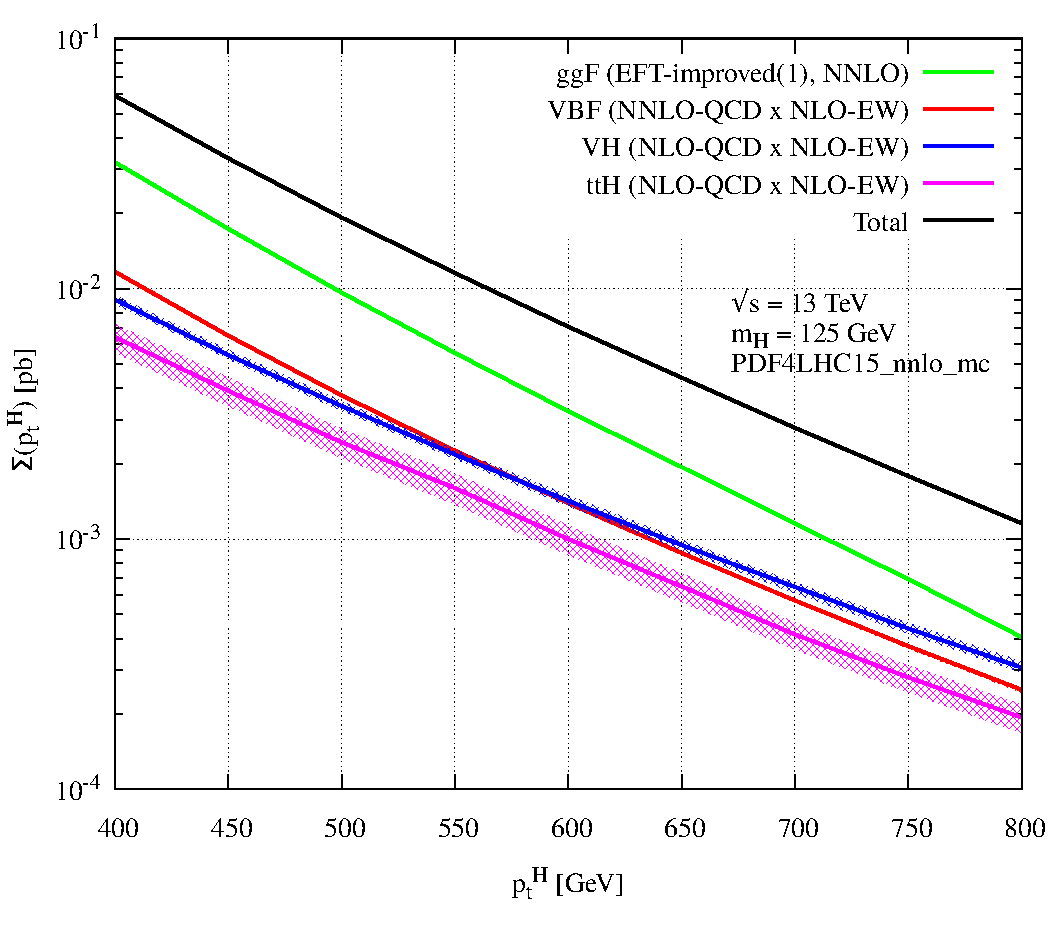
\includegraphics[width=0.45\textwidth]{\main/section2/plots/13TeV.pdf}~
    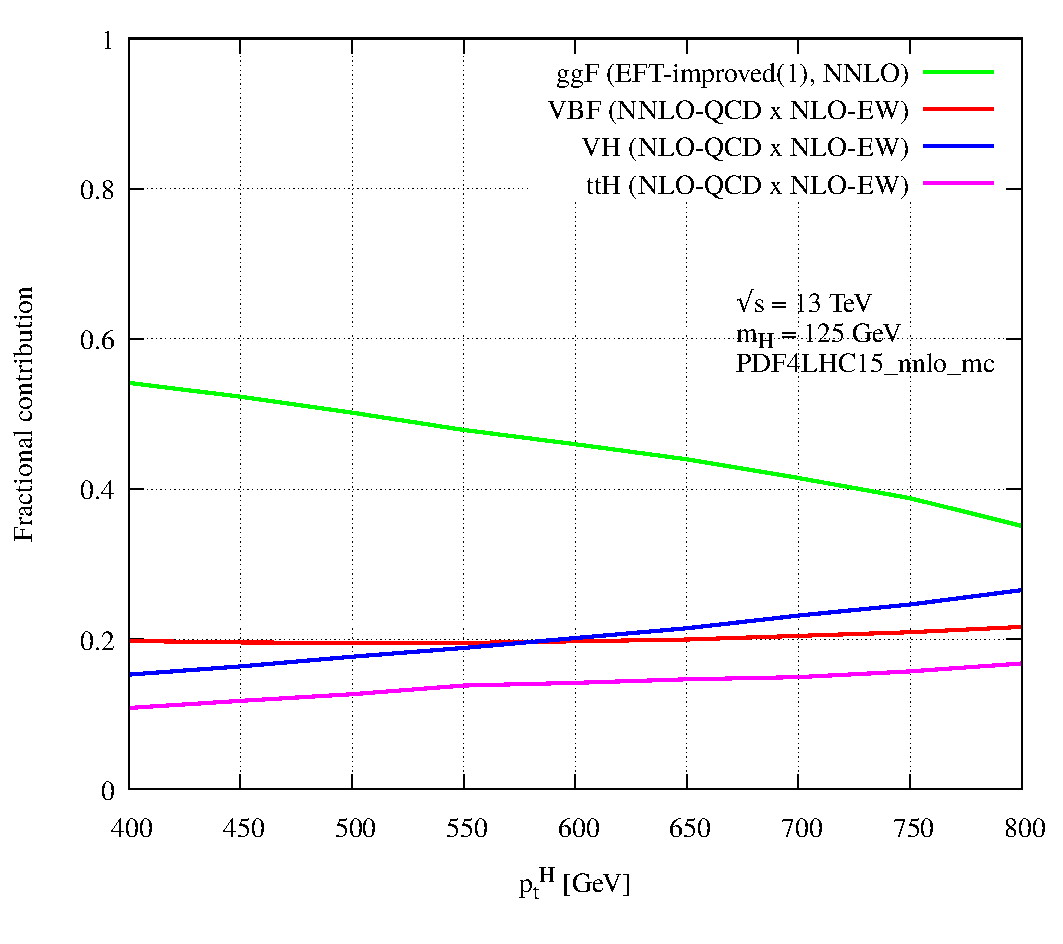
\includegraphics[width=0.45\textwidth]{\main/section2/plots/13TeV-ratio.pdf}
    \caption{
    Boosted Higgs prediction at the 13-TeV LHC. Left: cumulative transverse momentum distribution.
    Right: relative importance of different production mechanisms. See text for details. 
        \label{fig:boosted13}}
        \end{center}
\end{figure}
The $ggF$ prediction is obtained by rescaling the exact NLO with the NNLO $K-$factor in the $m_t\to\infty$
approximation, and it does not contain EW corrections. The VBF and VH predictions include NNLO QCD
and NLO EW corrections, while the $t\bar t H$ prediction includes NLO QCD and EW corrections. In
Fig.~\ref{fig:boosted13}(right), we show the relative importance of the different production mechanisms.\footnote{
The small feature around $p_t\sim 750~{\rm GeV}$ in the $ggF$ channel is due to lack of statistics in the
theoretical simulation and it is not a genuine physical feature.}
As it is well known, at high $p_t$ the $ggF$ channel becomes somewhat less dominant. Still, radiative
corrections strongly enhance this channel, which remains the dominant one in the TeV region. A very similar picture is expected for the HL-LHC. 

Figs.~\ref{fig:boosted27-LO} and~\ref{fig:boosted27} show similar predictions for the HE-LHC. In Fig.~\ref{fig:boosted27-LO}, all predictions are LO. 
\begin{figure}[h]
\begin{center}
    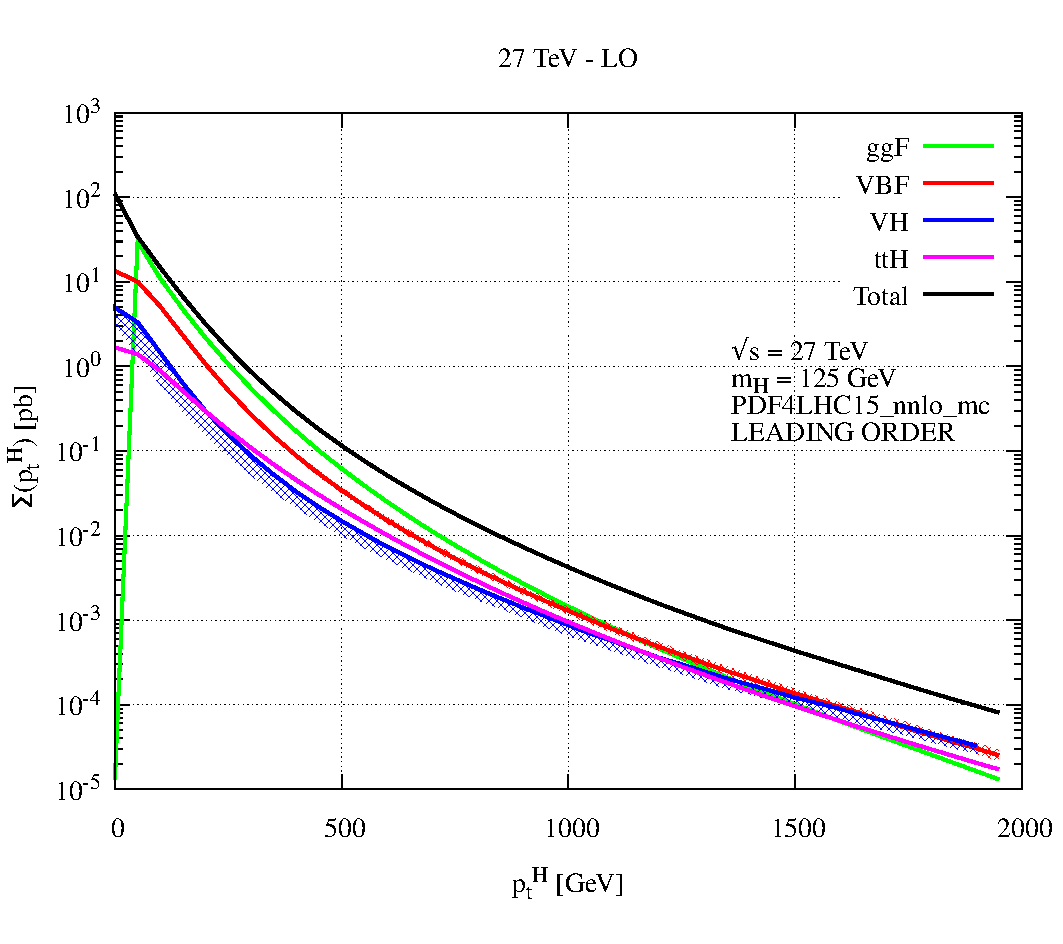
\includegraphics[width=0.45\textwidth]{\main/section2/plots/27TeV-LO.pdf}~
    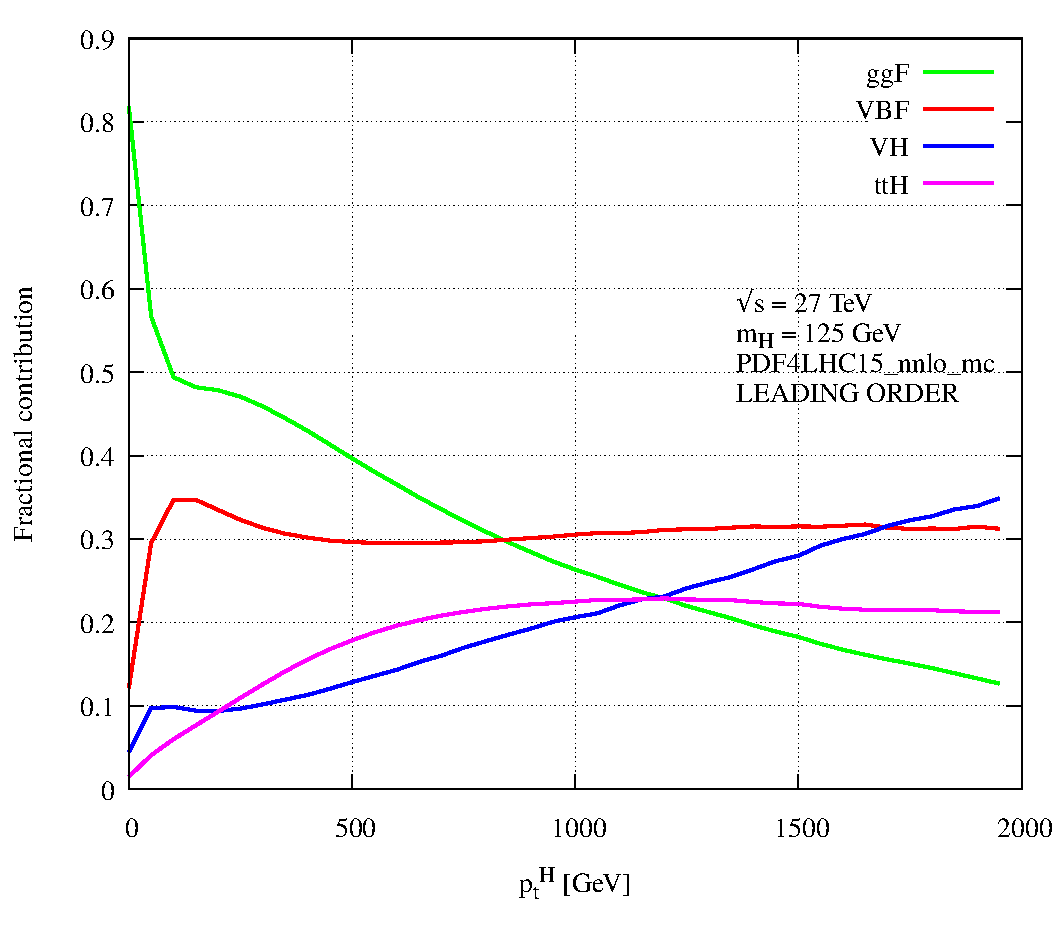
\includegraphics[width=0.45\textwidth]{\main/section2/plots/27TeV-LO-ratio.pdf}
    \caption{
    LO boosted Higgs prediction at the 27-TeV LHC. Left: cumulative transverse momentum distribution.
    Right: relative importance of different production mechanisms. See text for details. 
        \label{fig:boosted27-LO}}
        \end{center}
\end{figure}
\begin{figure}[h]
\begin{center}
    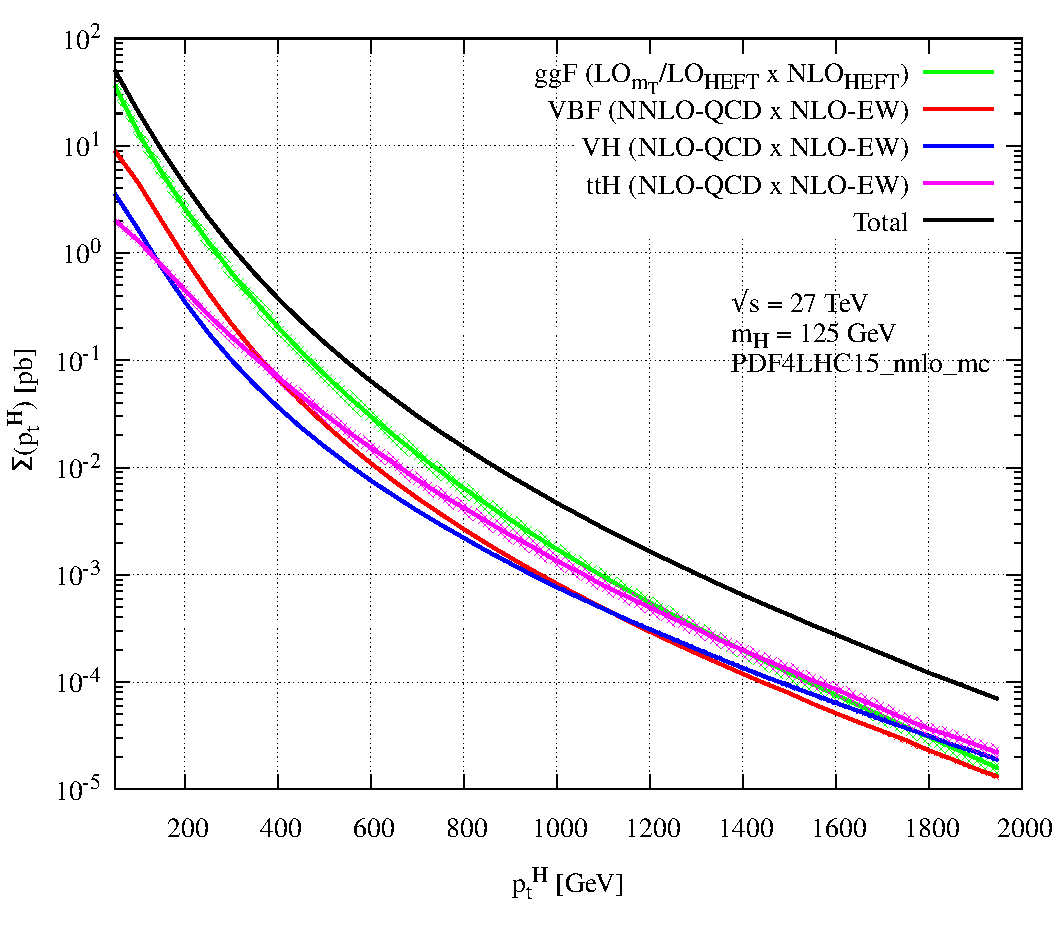
\includegraphics[width=0.45\textwidth]{\main/section2/plots/27TeV.pdf}~
    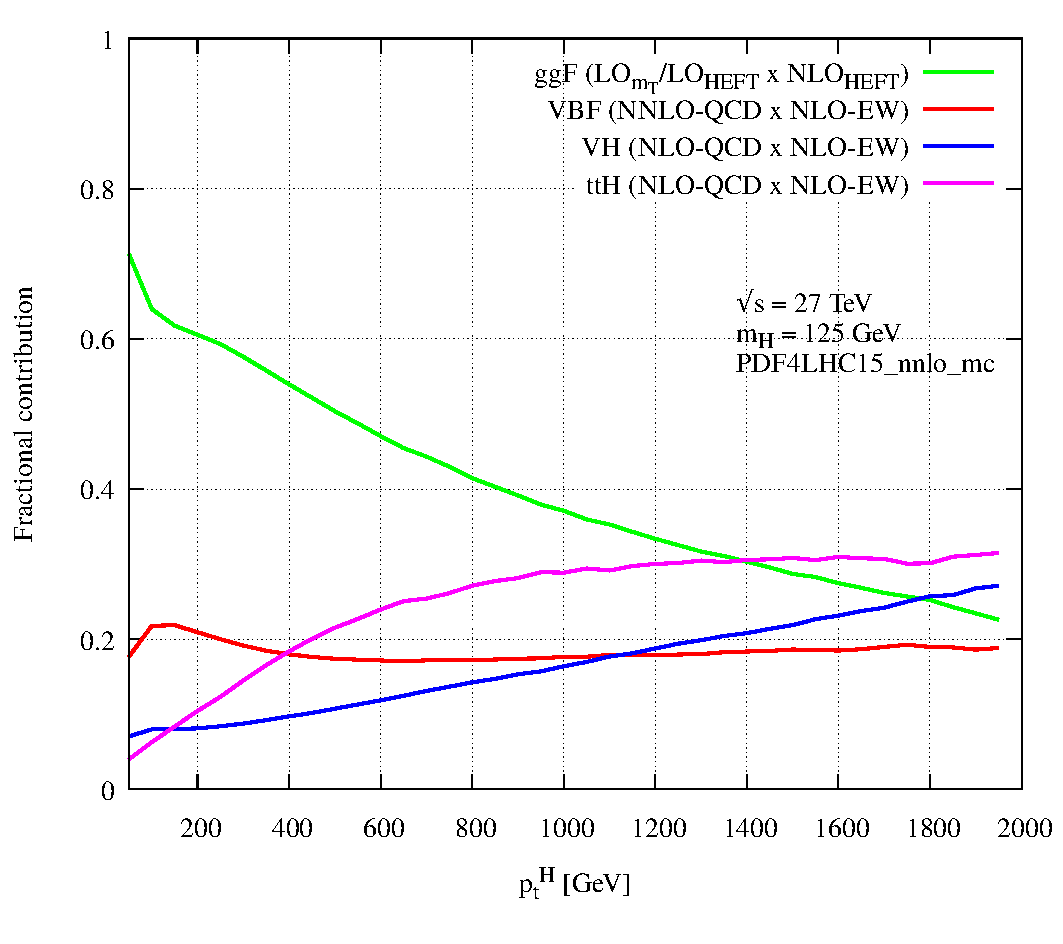
\includegraphics[width=0.45\textwidth]{\main/section2/plots/27TeV-ratio.pdf}
    \caption{
    Boosted Higgs prediction at the 27-TeV LHC, including radiative corrections. Left: cumulative transverse momentum distribution.
    Right: relative importance of different production mechanisms. See text for details. 
        \label{fig:boosted27}}
        \end{center}
\end{figure}
At high $p_t$, the $ggF$ channel become subdominant compared to the other ones. VBF becomes the dominant channel around  $p_t\sim 1~{\rm TeV}$, 
and VH around $p_t\sim 2~{\rm TeV}$. In the TeV region, the $t\bar t H$ channel becomes larger than $ggF$. 

This picture is however significantly altered by radiative correction, whose size and impact is very different for different channels. 
This is shown in Fig.~\ref{fig:boosted27}, where predictions include radiative corrections. More precisely, the VBF, VH and $t\bar t H$ 
predictions have the same accuracy of the ones in Fig.~\ref{fig:boosted13}. The $ggF$ prediction contains exact LO mass effects rescaled
by the NLO $K-$factor in the $m_t$ approximation. This is expected to provide an excellent approximation of the exact NLO result. 
Radiative correction enhance the relative importance of the $ggF$ and $t\bar t H$ channels, which still dominate over VBF well into the
multi-TeV region. At large $p_t \sim 1.5~{\rm TeV}$, the $t\bar t H$ channel becomes the dominant one. 

Obtaining accurate and precise theoretical predictions in the boosted region is very challenging. Nevertheless, it is natural
to expect progress in the timescale for the HL and HE LHC upgrades. This would allow for a proper scrutiny of the structure of
Higgs interactions in the multi-TeV regime. 

\subsubsection{Dependence of gluon-fusion cross section  at $14$ and $27$ TeV on $m_H$}
\label{sec:ggFmhdep}
The dependence of the inclusive gluon-fusion cross-section on the Higgs boson mass is shown in
Tables~\ref{ggF:14TeV} and~\ref{ggF:27TeV}, for $pp$ collisions at $\sqrt{s}=14$ and 27~TeV, respectively.
\begin{table}[!h]
\begin{center}
\begin{equation}
\begin{array}{|c|c|c|c|c|c|c|}
 \hline
 m_H  \text{ [GeV]}&\text{Cross Section [pb]}&\text{+ $\delta$Th. [\%]}&\text{- $\delta$Th. [\%]}&\pm\delta\text{(PDF+$\alpha_S$) [\%]}& \pm\delta\text{$\alpha_S$ [\%]} & \pm\delta\text{ PDF [\%]}  \\
\hline 
125.09 & 54.72 & 4.29 & -6.46 & 3.20 & 2.61 & 1.85\\
\hline 
124.59 & 55.10 & 4.29 & -6.48 & 3.20 & 2.61 & 1.86\\
\hline 
125.59 & 54.34 & 4.28 & -6.45 & 3.20 & 2.61 & 1.85\\
\hline 
120.00 & 58.85 & 4.37 & -6.61 & 3.23 & 2.63 & 1.87\\
\hline 
120.50 & 58.42 & 4.37 & -6.60 & 3.22 & 2.63 & 1.87\\
\hline 
121.00 & 58.00 & 4.36 & -6.58 & 3.22 & 2.63 & 1.87\\
\hline 
121.50 & 57.56 & 4.35 & -6.57 & 3.22 & 2.62 & 1.86\\
\hline 
122.00 & 57.15 & 4.34 & -6.55 & 3.22 & 2.62 & 1.86\\
\hline 
122.50 & 56.75 & 4.33 & -6.54 & 3.21 & 2.62 & 1.86\\
\hline 
123.00 & 56.35 & 4.32 & -6.52 & 3.21 & 2.62 & 1.86\\
\hline 
123.50 & 55.95 & 4.31 & -6.51 & 3.21 & 2.61 & 1.86\\
\hline 
124.00 & 55.56 & 4.30 & -6.49 & 3.21 & 2.61 & 1.86\\
\hline 
124.10 & 55.48 & 4.30 & -6.49 & 3.20 & 2.61 & 1.86\\
\hline 
124.20 & 55.41 & 4.30 & -6.49 & 3.20 & 2.61 & 1.86\\
\hline 
124.30 & 55.33 & 4.30 & -6.49 & 3.20 & 2.61 & 1.86\\
\hline 
124.40 & 55.25 & 4.30 & -6.48 & 3.20 & 2.61 & 1.86\\
\hline 
124.50 & 55.17 & 4.30 & -6.48 & 3.20 & 2.61 & 1.86\\
\hline 
124.60 & 55.10 & 4.29 & -6.48 & 3.20 & 2.61 & 1.86\\
\hline 
124.70 & 55.02 & 4.29 & -6.47 & 3.20 & 2.61 & 1.86\\
\hline 
124.80 & 54.94 & 4.29 & -6.47 & 3.20 & 2.61 & 1.86\\
\hline 
124.90 & 54.86 & 4.29 & -6.47 & 3.20 & 2.61 & 1.86\\
\hline 
125.00 & 54.79 & 4.29 & -6.47 & 3.20 & 2.61 & 1.86\\
\hline 
125.10 & 54.71 & 4.29 & -6.46 & 3.20 & 2.61 & 1.85\\
\hline 
125.20 & 54.64 & 4.28 & -6.46 & 3.20 & 2.61 & 1.85\\
\hline 
125.30 & 54.56 & 4.28 & -6.46 & 3.20 & 2.61 & 1.85\\
\hline 
125.40 & 54.48 & 4.28 & -6.45 & 3.20 & 2.61 & 1.85\\
\hline 
125.50 & 54.41 & 4.28 & -6.45 & 3.20 & 2.61 & 1.85\\
\hline 
125.60 & 54.33 & 4.28 & -6.45 & 3.20 & 2.61 & 1.85\\
\hline 
125.70 & 54.26 & 4.28 & -6.44 & 3.20 & 2.61 & 1.85\\
\hline 
125.80 & 54.18 & 4.27 & -6.44 & 3.20 & 2.60 & 1.85\\
\hline 
125.90 & 54.11 & 4.27 & -6.44 & 3.20 & 2.60 & 1.85\\
\hline 
126.00 & 54.03 & 4.27 & -6.44 & 3.20 & 2.60 & 1.85\\
\hline 
126.50 & 53.66 & 4.26 & -6.42 & 3.19 & 2.60 & 1.85\\
\hline 
127.00 & 53.29 & 4.25 & -6.41 & 3.19 & 2.60 & 1.85\\
\hline 
127.50 & 52.92 & 4.25 & -6.40 & 3.19 & 2.60 & 1.85\\
\hline 
128.00 & 52.56 & 4.24 & -6.38 & 3.19 & 2.60 & 1.85\\
\hline 
128.50 & 52.20 & 4.23 & -6.37 & 3.18 & 2.59 & 1.85\\
\hline 
129.00 & 51.85 & 4.22 & -6.35 & 3.18 & 2.59 & 1.85\\
\hline 
129.50 & 51.50 & 4.21 & -6.34 & 3.18 & 2.59 & 1.84\\
\hline 
130.00 & 51.15 & 4.20 & -6.33 & 3.18 & 2.59 & 1.84\\
\hline
\end{array}
\nonumber
\end{equation}
\end{center}
\caption{The gluon-fusion cross-section in $pp$ collisions at $\sqrt{s}=14$~TeV, for different values of the Higgs boson mass $m_H$. \label{ggF:14TeV}}
\end{table}

\begin{table}[!h]
\begin{center}
\begin{equation}
\begin{array}{|c|c|c|c|c|c|c|}
 \hline
 m_H  \text{ [GeV]}&\text{Cross Section [pb]}&\text{+ $\delta$Th. [\%]}&\text{- $\delta$Th. [\%]}&\pm\delta\text{(PDF+$\alpha_S$) [\%]}& \pm\delta\text{$\alpha_S$ [\%]} & \pm\delta\text{ PDF [\%]}  \\
\hline 
125.09 & 146.65 & 4.53 & -6.43 & 3.30 & 2.66 & 1.95\\
\hline 
124.59 & 147.55 & 4.55 & -6.45 & 3.30 & 2.67 & 1.95\\
\hline 
125.59 & 145.75 & 4.52 & -6.42 & 3.30 & 2.66 & 1.95\\
\hline 
120.00 & 156.35 & 4.64 & -6.60 & 3.33 & 2.69 & 1.97\\
\hline 
120.50 & 155.36 & 4.63 & -6.58 & 3.33 & 2.69 & 1.97\\
\hline 
121.00 & 154.36 & 4.62 & -6.56 & 3.33 & 2.69 & 1.97\\
\hline 
121.50 & 153.38 & 4.61 & -6.55 & 3.32 & 2.68 & 1.96\\
\hline 
122.00 & 152.41 & 4.60 & -6.54 & 3.32 & 2.68 & 1.96\\
\hline 
122.50 & 151.45 & 4.59 & -6.52 & 3.32 & 2.68 & 1.96\\
\hline 
123.00 & 150.50 & 4.58 & -6.50 & 3.31 & 2.68 & 1.96\\
\hline 
123.50 & 149.56 & 4.57 & -6.49 & 3.31 & 2.67 & 1.96\\
\hline 
124.00 & 148.64 & 4.56 & -6.47 & 3.31 & 2.67 & 1.95\\
\hline 
124.10 & 148.45 & 4.56 & -6.47 & 3.31 & 2.67 & 1.95\\
\hline 
124.20 & 148.27 & 4.56 & -6.46 & 3.31 & 2.67 & 1.95\\
\hline 
124.30 & 148.08 & 4.55 & -6.46 & 3.31 & 2.67 & 1.95\\
\hline 
124.40 & 147.90 & 4.55 & -6.46 & 3.31 & 2.67 & 1.95\\
\hline 
124.50 & 147.72 & 4.55 & -6.46 & 3.31 & 2.67 & 1.95\\
\hline 
124.60 & 147.53 & 4.55 & -6.45 & 3.30 & 2.67 & 1.95\\
\hline 
124.70 & 147.35 & 4.54 & -6.45 & 3.30 & 2.67 & 1.95\\
\hline 
124.80 & 147.17 & 4.54 & -6.44 & 3.30 & 2.67 & 1.95\\
\hline 
124.90 & 146.99 & 4.54 & -6.44 & 3.30 & 2.67 & 1.95\\
\hline 
125.00 & 146.81 & 4.54 & -6.44 & 3.30 & 2.67 & 1.95\\
\hline 
125.10 & 146.63 & 4.53 & -6.43 & 3.30 & 2.66 & 1.95\\
\hline 
125.20 & 146.45 & 4.53 & -6.43 & 3.30 & 2.66 & 1.95\\
\hline 
125.30 & 146.27 & 4.53 & -6.43 & 3.30 & 2.66 & 1.95\\
\hline 
125.40 & 146.09 & 4.53 & -6.42 & 3.30 & 2.66 & 1.95\\
\hline 
125.50 & 145.91 & 4.52 & -6.42 & 3.30 & 2.66 & 1.95\\
\hline 
125.60 & 145.73 & 4.52 & -6.42 & 3.30 & 2.66 & 1.95\\
\hline 
125.70 & 145.55 & 4.52 & -6.41 & 3.30 & 2.66 & 1.95\\
\hline 
125.80 & 145.37 & 4.52 & -6.41 & 3.30 & 2.66 & 1.95\\
\hline 
125.90 & 145.20 & 4.52 & -6.41 & 3.30 & 2.66 & 1.95\\
\hline 
126.00 & 145.02 & 4.51 & -6.40 & 3.30 & 2.66 & 1.95\\
\hline 
126.50 & 144.14 & 4.50 & -6.39 & 3.29 & 2.66 & 1.94\\
\hline 
127.00 & 143.26 & 4.49 & -6.37 & 3.29 & 2.66 & 1.94\\
\hline 
127.50 & 142.40 & 4.48 & -6.36 & 3.29 & 2.65 & 1.94\\
\hline 
128.00 & 141.54 & 4.48 & -6.34 & 3.28 & 2.65 & 1.94\\
\hline 
128.50 & 140.69 & 4.47 & -6.33 & 3.28 & 2.65 & 1.94\\
\hline 
129.00 & 139.84 & 4.46 & -6.31 & 3.28 & 2.65 & 1.93\\
\hline 
129.50 & 139.00 & 4.46 & -6.30 & 3.27 & 2.64 & 1.93\\
\hline 
130.00 & 138.18 & 4.45 & -6.29 & 3.27 & 2.64 & 1.93\\
 \hline
\end{array}
\nonumber
\end{equation}
\end{center}
\caption{The gluon-fusion cross-section in $pp$ collisions at $\sqrt{s}=27$~TeV, for different values of the Higgs boson mass $m_H$. \label{ggF:27TeV}}
\end{table}
 

